\documentclass[conference,10pt,a4paper]{IEEEtran}
\usepackage[T1]{fontenc}
\usepackage{mathptmx}
\usepackage{graphicx}
\usepackage{booktabs}
\usepackage{microtype}
\usepackage[hidelinks]{hyperref}

\begin{document}

\title{Sensitivity of NCCL Collectives to Emulated Network Impairments: A Two-Node Study}
\author{\IEEEauthorblockN{Lisa Polupanova}
\IEEEauthorblockA{Semester Thesis, ETH Z\"urich}}
\maketitle

\begin{abstract}
We measure how the collective completion time (CCT) of NCCL AllReduce and SendRecv between two GPU nodes reacts to added latency, jitter, packet loss and bandwidth caps emulated with Linux \texttt{netem}. Up to 100\,ms of added delay, AllReduce slows down by the same factor for 32, 64 and 128\,MiB messages (2.2$\times$ at 100\,ms), showing that delay reduces throughput rather than adding a fixed cost. Beyond that, performance collapses: 200\,ms of delay or 6\,ms of jitter make AllReduce 15--20$\times$ slower. Random loss up to 1\,\% costs at most 1.5$\times$. Under bandwidth caps, SendRecv follows the ideal size/rate bound, whereas AllReduce becomes erratic and up to 6$\times$ slower than that bound.
\end{abstract}

\section{Introduction}
Training across data centres or clouds moves gradient and activation traffic from dedicated interconnects onto shared, lossy wide-area links. Collective libraries such as NCCL are tuned for low-latency fabrics; how their completion time degrades on commodity TCP networks determines whether such deployments are viable. This report isolates that question for the two primitives that dominate data- and pipeline-parallel training: AllReduce and point-to-point SendRecv.

\section{Experimental Setup}
\textbf{Testbed.} Two cloud VMs, each with one NVIDIA Tesla V100-SXM2-16GB, connected over Ethernet. Without InfiniBand, NCCL (2.29.3) uses its socket transport, i.e.\ TCP. Unimpaired, a 32\,MiB transfer completes in 276\,ms, an effective rate of 0.97\,Gbit/s.

\textbf{Workload.} We run \texttt{all\_reduce\_perf} (float sum) and \texttt{sendrecv\_perf} from nccl-tests 2.18.5, launched with Open MPI, for message sizes $S\in\{32, 64, 128\}$\,MiB. The CCT is the mean out-of-place time per operation reported by nccl-tests over 20 timed iterations after warm-up (bandwidth sweeps: 5 iterations, 1 warm-up). With two ranks, a ring AllReduce sends $S/2$ in its reduce-scatter and $S/2$ in its all-gather phase, so both operations move exactly $S$ bytes per direction; their unimpaired CCTs are indeed equal (276/559/1106\,ms vs.\ 276/552/1107\,ms).

\textbf{Impairments.} \texttt{tc netem} on the egress interface of node~0 applies one factor at a time: delay 0--200\,ms; jitter 0--6\,ms (uniform) on a fixed 10\,ms delay; random loss 0--1\,\%; rate caps of 100--1000\,Mbit/s. Each point is a single run. We report the slowdown, $\mathrm{CCT}/\mathrm{CCT}_0$, where $\mathrm{CCT}_0$ is the unimpaired CCT of the same operation and size.

\section{Results}
\begin{figure}[t]
\centering
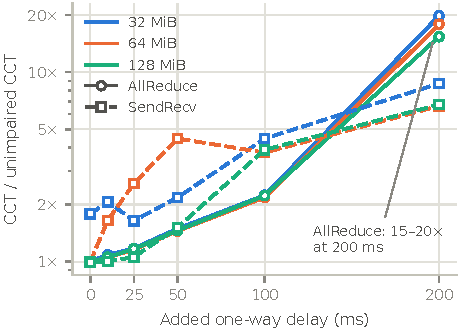
\includegraphics[width=\columnwidth]{fig_latency.pdf}
\caption{Slowdown under added one-way delay (log scale). AllReduce curves for all three sizes coincide up to 100\,ms. The SendRecv 32\,MiB point at 0\,ms (1.8$\times$) is a run-to-run outlier of the same unimpaired configuration.}
\label{fig:latency}
\end{figure}

\textbf{Latency (Fig.~\ref{fig:latency}).} For AllReduce the slowdown is independent of the message size: 1.17$\times$ at 25\,ms, 1.45--1.49$\times$ at 50\,ms and 2.18--2.24$\times$ at 100\,ms for 32, 64 and 128\,MiB alike. Equivalently, every millisecond of delay adds 3.4, 6.7 and 13.6\,ms to the CCT, in proportion to $S$. Delay therefore lowers the achieved throughput rather than adding a per-message constant, as expected for window-limited TCP, whose rate scales with window/RTT. At 200\,ms the AllReduce CCT jumps to 15--20$\times$ the baseline. SendRecv degrades more irregularly: 3.8--4.5$\times$ at 100\,ms but only 6.6--8.7$\times$ at 200\,ms, i.e.\ without the AllReduce collapse. Its noisy low-delay points (e.g.\ 64\,MiB is slower at 50 than at 100\,ms) indicate substantial run-to-run variance.

\begin{figure*}[t]
\centering
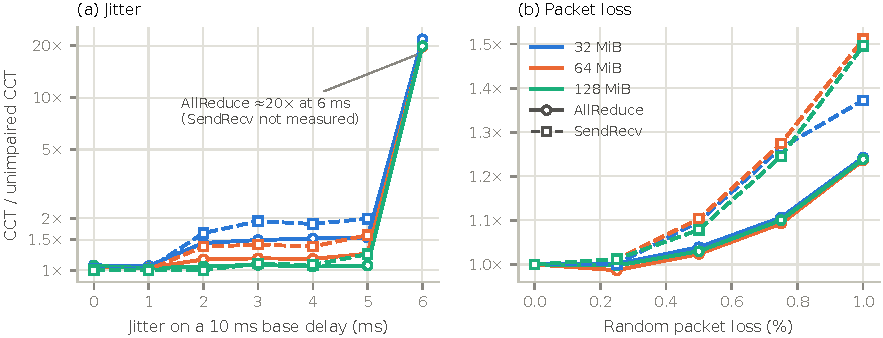
\includegraphics[width=\textwidth]{fig_jitter_loss.pdf}
\caption{Slowdown under (a) jitter on top of a 10\,ms base delay (log scale) and (b) random packet loss. Line colour: message size; solid/circles: AllReduce; dashed/squares: SendRecv.}
\label{fig:jitterloss}
\end{figure*}

\textbf{Jitter (Fig.~\ref{fig:jitterloss}a).} Up to 1\,ms of jitter has no measurable effect beyond the 10\,ms base delay. Between 2 and 5\,ms the cost depends strongly on the message size: AllReduce slows down by 1.44--1.55$\times$ at 32\,MiB, 1.15--1.25$\times$ at 64\,MiB and only 1.03--1.07$\times$ at 128\,MiB; SendRecv reacts more (up to 1.99$\times$ at 32\,MiB). A per-message stall that larger transfers amortise would explain this ordering. At 6\,ms all AllReduce sizes collapse to $\approx$20$\times$. We attribute the cliff to packet reordering by \texttt{netem}: once delay variations exceed the inter-packet spacing by enough, TCP interprets reordering as loss and repeatedly shrinks its congestion window. SendRecv was not measured at 6\,ms.

\textbf{Packet loss (Fig.~\ref{fig:jitterloss}b).} Loss of 0.25\,\% is negligible. At 1\,\%, AllReduce is 1.24$\times$ slower for every size, again a size-independent throughput effect, while SendRecv is more sensitive (1.37--1.51$\times$). Among the tested factors, loss is the most benign.

\begin{figure}[t]
\centering
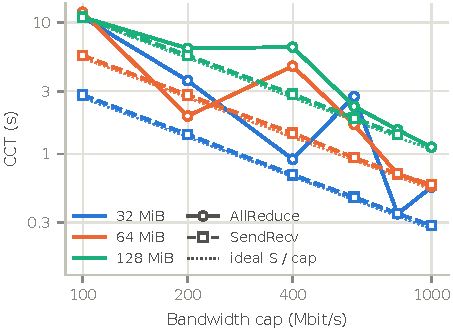
\includegraphics[width=\columnwidth]{fig_bandwidth.pdf}
\caption{CCT under bandwidth caps (log--log). Dotted lines: ideal $S/\mathrm{cap}$, which both operations should reach since each moves $S$ bytes per direction.}
\label{fig:bandwidth}
\end{figure}

\textbf{Bandwidth (Fig.~\ref{fig:bandwidth}).} SendRecv tracks the ideal $S/\mathrm{cap}$ within about 5\,\% over the whole range (32\,MiB: 2.81\,s vs.\ 2.68\,s at 100\,Mbit/s, 0.285\,s vs.\ 0.268\,s at 1\,Gbit/s), which also confirms that the emulated rate is accurate. AllReduce does not: its CCT is non-monotonic in the cap and exceeds the bound by up to 6.1$\times$ (32\,MiB at 600\,Mbit/s: 2.74\,s vs.\ 0.45\,s). Since both operations carry the same bytes, the difference must come from how AllReduce interleaves its two phases with a rate-limited queue; with only five iterations per point, however, we cannot separate this from measurement variance.

\section{Discussion and Limitations}
Three regimes emerge. (i) Moderate delay ($\le$100\,ms) and loss ($\le$1\,\%) slow collectives by a size-independent factor of at most $\approx$2.2$\times$; larger gradient buckets do not help, because the penalty is per byte. (ii) Moderate jitter mainly hurts small messages, which favours fewer, larger transfers. (iii) Long delays and jitter at or above 6\,ms push default TCP into a collapse an order of magnitude worse, which is a configuration rather than a hardware limit: larger socket buffers or more NCCL sockets per connection are the obvious next step.

The study has clear limits. Every point is a single run, so non-monotonic points (SendRecv under delay, AllReduce under rate caps) cannot be told apart from noise; repetitions with confidence intervals are needed. nccl-tests prints times of 10\,s and more with only two significant digits (e.g.\ \texttt{1.1e+07}\,$\mu$s). Impairments act only on node~0's egress, kernel TCP settings were left at their defaults, and all results come from a single VM pair. Rate caps of 10 and 50\,Mbit/s did not produce results and are absent.

\end{document}
